\documentclass[11pt]{scrartcl}

\title{Systemtest}
\author{Silvan Adrian \\ Fabian Binna}
\date{\today{}}

\usepackage[ngerman]{babel}
\usepackage[automark]{scrpage2}
\usepackage[colorlinks = true,
linkcolor = black]{hyperref}
\usepackage{color}
\usepackage[normalem]{ulem}
\usepackage{scrpage2}
\usepackage{graphicx}
\usepackage{tabularx}
\graphicspath{ {../22_Grafiken/01_Logo/}{images/}{images/1.Sprint/}{images/2.Sprint/}{images/3.Sprint/}{../../22_Grafiken/01_Logo/} }
\pagestyle{scrheadings}

\clearscrheadfoot
\ihead{
\includegraphics[scale=0.3]{SDDC}}
\ohead{Projekt: SDDC}
\ifoot{Systemtest}
\cfoot{Version: 1.00}
\ofoot{Datum: 2. November 2015}
\setheadsepline{0.5pt}
\setfootsepline{0.5pt}

\usepackage{ucs}
\usepackage[utf8]{inputenc}
\usepackage[T1]{fontenc}


\begin{document}
\def\arraystretch{1.5}
\begin{titlepage}
\begin{center}
\vspace{10em}

\includegraphics[scale=2]{SDDC}
\vspace{10em}
\end{center}
\begin{center}
\huge {Testprotokoll}\\
\huge {02.11.15 - Sprint 1}\\
\end{center}
\begin{center}
\vspace{10em}
\LARGE {Silvan Adrian} \\
\LARGE {Fabian Binna}
\end{center}

\end{titlepage}


\newpage
\tableofcontents
\newpage

\section{Test}
\subsection{Angaben zum Test}

\begin{tabularx}{\linewidth}{l l l}
\textbf{datum des Builds} & \textbf{Tester} & \textbf{datum der Testdurchführung}\\
\hline
02.11.15 & Silvan Adrian & 02.11.15

\end{tabularx}

\subsection{Zusammenfassung Ergebnis}
\begin{tabularx}{\linewidth}{l l l}
\textbf{Test durchgeführt?} & \textbf{Tests erfolgreich?} & \textbf{Tests fehlgeschalgen?}\\
\hline
5 (alle) & 5 (alle) & 0 \\
\hline
\end{tabularx}


\subsection{Ergebnisse Tests}
\begin{tabularx}{\linewidth}{l l l}
\textbf{Was} & \textbf{Ok? / nicht OK?} & \textbf{Aufgetretene Fehler}\\
\hline
\textbf{Unit-Tests} & {\color{green} OK}  & keine\\
\hline
Systemtest 1: & & \\
\textbf{Testservice abonnieren} & {\color{green} OK} & keine\\
\hline
Systemtest 2: & & \\
\textbf{Testservice kündigen} & {\color{green} OK}  & keine\\
\hline
Systemtest 3: & & \\
\textbf{Abonnierte Services anzeigen} & {\color{green} OK}  & keine\\
\hline
Systemtest 4: & & \\
\textbf{Verfügbare Services anzeigen} & {\color{green} OK}  & keine\\
\hline



\end{tabularx}

\newpage

\section{Metriken}
Die abschliessenden Metriken vom Sprint aus SonarQube.
\subsection{Projekt in Zahlen}
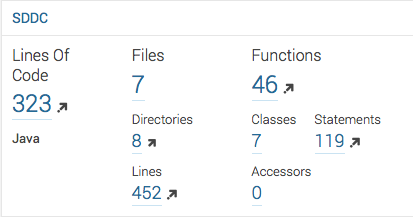
\includegraphics[]{loc}

\subsection{Unit Tests Coverage}
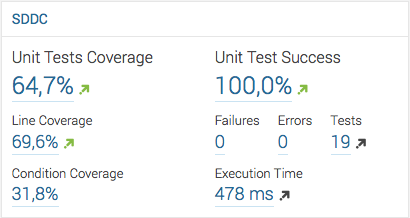
\includegraphics[]{coverage}

\subsection{Coverage Verteilung auf einzelne Dateien}
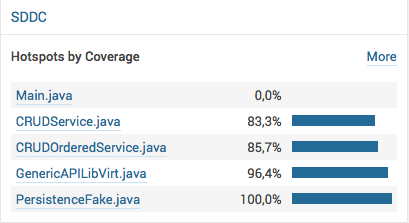
\includegraphics[]{covergaeperfile}

\subsection{Findbugs Issues}
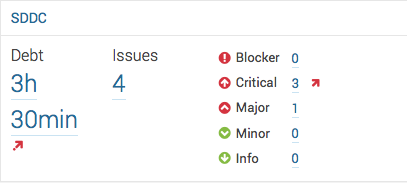
\includegraphics[]{issues}
\subsubsection{Issues}
\textbf{HashCode}\\
Da es isch hierbei nur um einen Persistance Fake handelt wurde drauf verzichtet 
das Issue zu beheben und wird im nächsten Sprint sowieso entfernt.
\newline
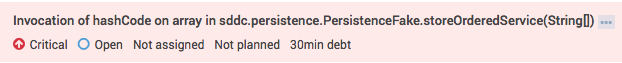
\includegraphics[width=\textwidth]{hashcode}
\newline
\textbf{Encoding}\\
Issue besteht im Main File. welches im nächsten Sprint nicht mehr so existiert.
\newline
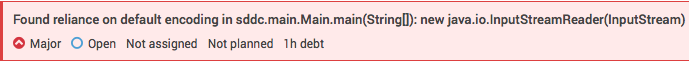
\includegraphics[width=\textwidth]{encoding}
\newline
\textbf{Infiniteloop}\\
Für die Konsolen Eingaben wurde ein Infinite Loop erstellt, welcher es einem 
erlaubt mehrmals Eingaben zu machen.
\newline
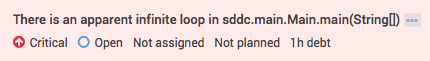
\includegraphics[width=\textwidth]{infiniteloop}
\newline
\textbf{Null Check}\\
Ebenfalls im Main java File, welches noch abgeändert und nicht mehr in dieser 
Konstellation existieren wird.
\newline
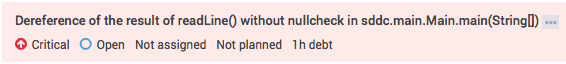
\includegraphics[width=\textwidth]{nullcheck}

\section{Kommentare}

Die Konsolen App bietet ganz einfach Eingaben und Möglichkeiten die Service 
abonnieren und kündigen zu können.
Verbesserungen werden im Code Review Dokument beschrieben.

\end{document}